\documentclass[tikz,border=0pt]{standalone}
% Shared look for the README diagrams. Colours are the app's own tokens (web/styles.css).
\usepackage[T1]{fontenc}
\usepackage[scaled=0.95]{helvet}
\renewcommand{\familydefault}{\sfdefault}
\usepackage{amsmath,amssymb}
\usepackage{tikz}
\usetikzlibrary{arrows.meta,positioning,fit,backgrounds,calc,shapes.geometric,shapes.symbols}

\definecolor{ink}{HTML}{15233F}
\definecolor{inksoft}{HTML}{3A4D6B}
\definecolor{paper}{HTML}{D9E7EF}
\definecolor{paperdeep}{HTML}{C6DAE6}
\definecolor{rule}{HTML}{9DB8CB}
\definecolor{safe}{HTML}{17643A}
\definecolor{safewash}{HTML}{D3EBDC}
\definecolor{caution}{HTML}{7A4F00}
\definecolor{cautionwash}{HTML}{F3DFA6}
\definecolor{danger}{HTML}{B0221B}
\definecolor{dangerwash}{HTML}{F7DCD9}
\definecolor{stop}{HTML}{8D0C0C}
\definecolor{stopwash}{HTML}{F6D4CF}
\definecolor{coral}{HTML}{FF8A80}
\definecolor{canvas}{HTML}{F7FAFC}

\newcommand{\modtitle}[1]{{\small\bfseries #1}}
\newcommand{\grouptag}[1]{{\scriptsize\bfseries\color{inksoft}\MakeUppercase{#1}}}

\tikzset{
  every node/.style={font=\footnotesize, text=ink},
  mod/.style={draw=ink, line width=0.7pt, fill=white, rounded corners=3pt, align=center,
              minimum height=1.25cm, inner sep=4pt},
  api/.style={mod, fill=paper},
  actor/.style={mod, fill=ink, text=white, minimum width=2.8cm},
  frame/.style={draw=rule, line width=0.8pt, dashed, rounded corners=6pt, inner sep=10pt},
  flow/.style={-{Stealth[length=6pt,width=5pt]}, line width=0.8pt, draw=ink},
  soft/.style={flow, draw=inksoft, dashed},
  halo/.style={preaction={draw=canvas, line width=4pt, -}},
  lab/.style={font=\scriptsize, text=inksoft, fill=canvas, inner sep=1.5pt},
  store/.style={cylinder, shape border rotate=90, aspect=0.18, draw=ink, line width=0.7pt,
                fill=paper, align=center, minimum height=1.35cm, inner sep=4pt},
}

% Light card behind everything (own layer, under the frames), so the SVG reads on GitHub's dark theme too.
\pgfdeclarelayer{card}
\pgfsetlayers{card,background,main}
\newcommand{\card}{%
  \begin{pgfonlayer}{card}
    \fill[canvas, rounded corners=10pt]
      ($(current bounding box.south west)+(-0.5,-0.5)$) rectangle ($(current bounding box.north east)+(0.5,0.5)$);
  \end{pgfonlayer}}
% code names without a bitmap typewriter font
\newcommand{\code}[1]{{\color{inksoft}\itshape #1}}
\begin{document}
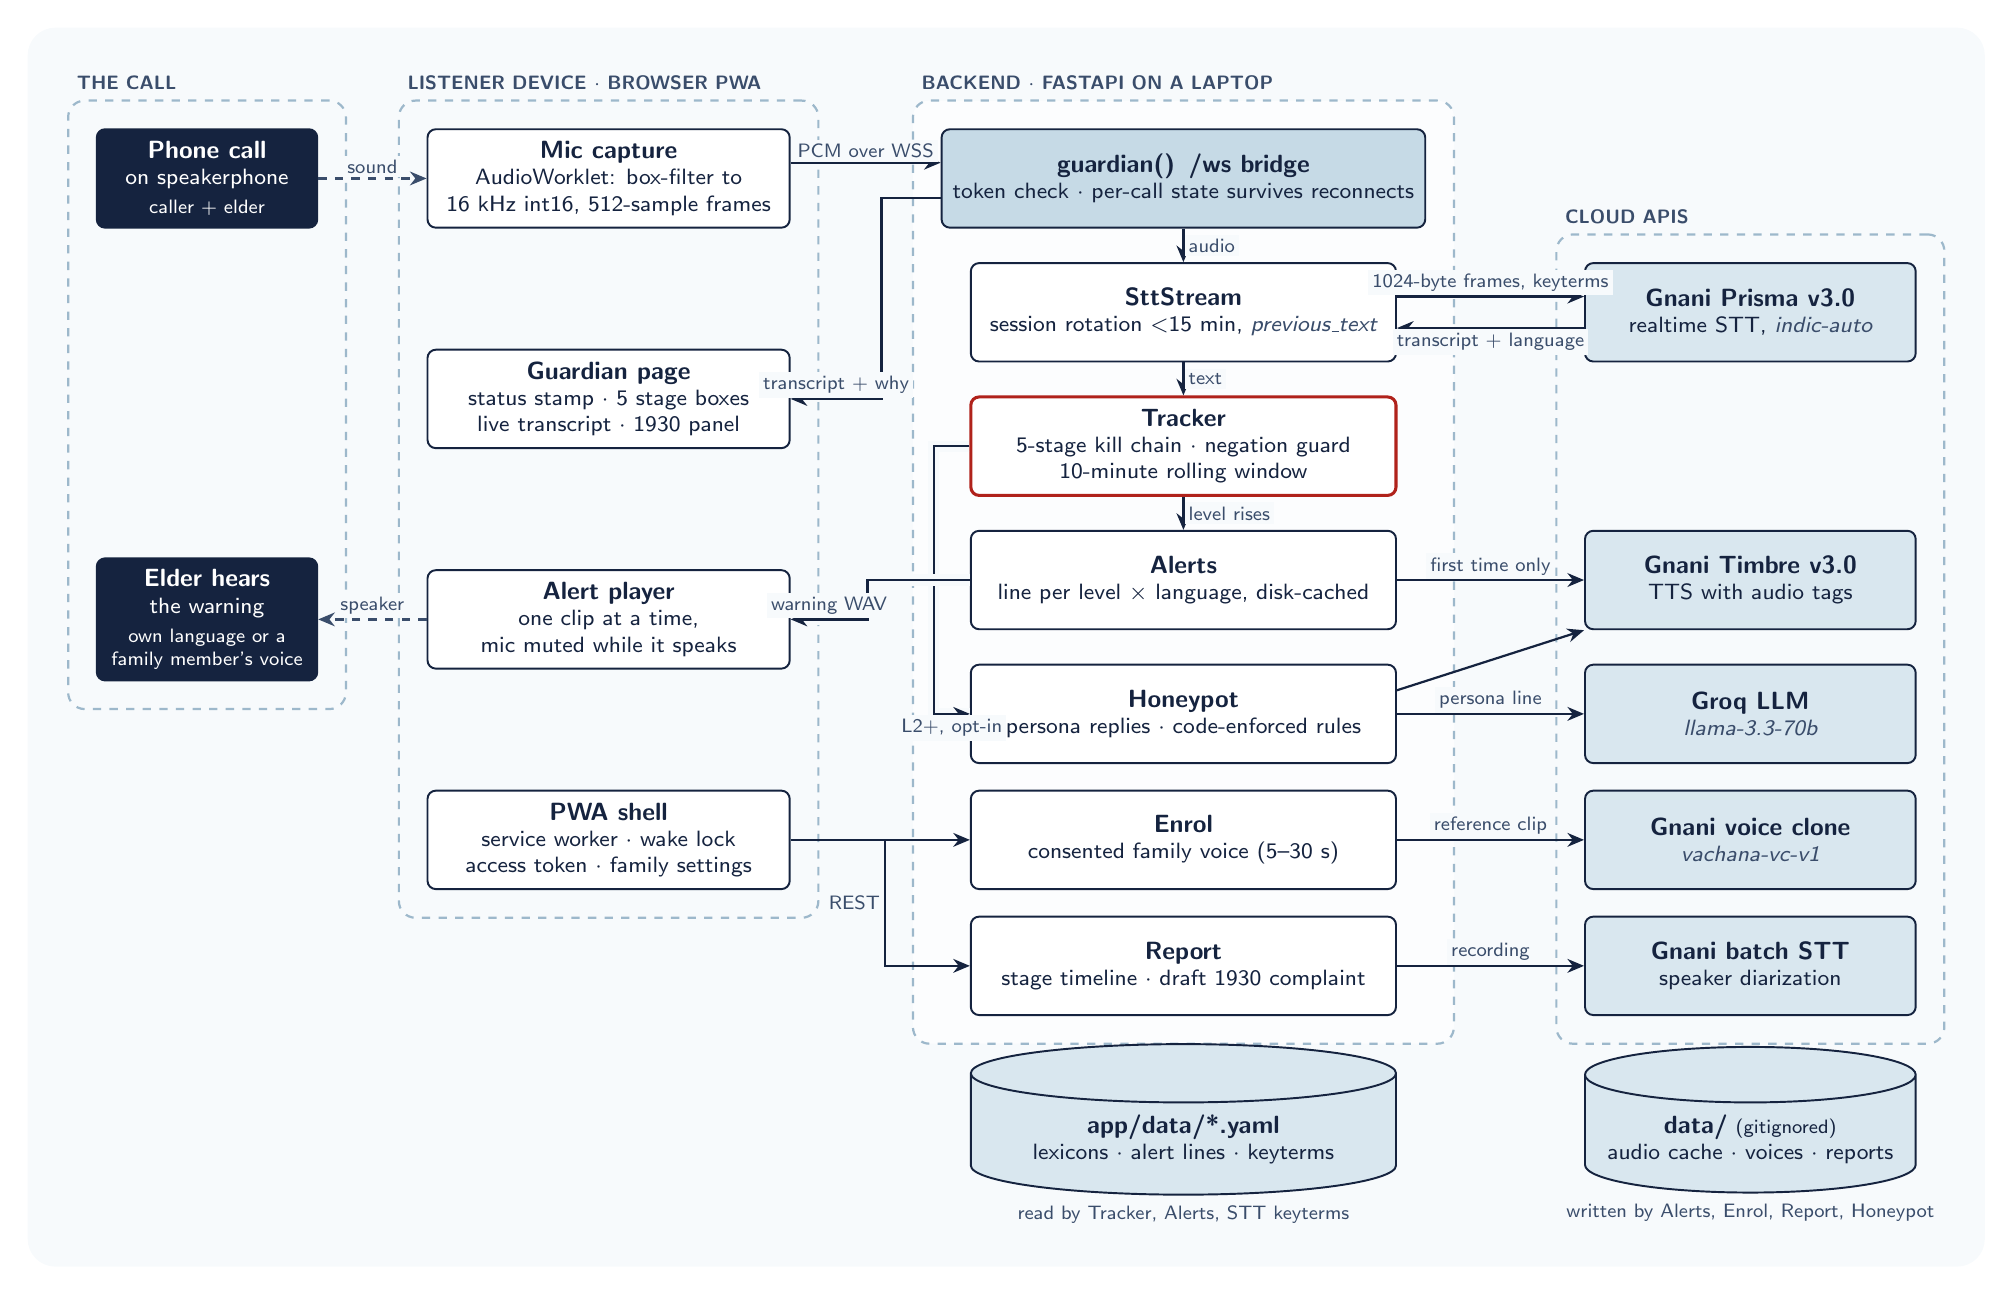
\begin{tikzpicture}[x=1cm,y=1cm]

% ---- call side --------------------------------------------------------------
\node[actor] (phone) at (1.6,11.2) {\modtitle{Phone call}\\on speakerphone\\[1pt]{\scriptsize caller + elder}};
\node[actor] (elder) at (1.6,5.6) {\modtitle{Elder hears}\\the warning\\[1pt]{\scriptsize own language or a}\\[-1pt]{\scriptsize family member's voice}};

% ---- listener device ----------------------------------------------------------
\begin{scope}[every node/.append style={mod, minimum width=4.6cm}]
  \node (mic)    at (6.7,11.2) {\modtitle{Mic capture}\\AudioWorklet: box-filter to\\16 kHz int16, 512-sample frames};
  \node (ui)     at (6.7,8.4)  {\modtitle{Guardian page}\\status stamp $\cdot$ 5 stage boxes\\live transcript $\cdot$ 1930 panel};
  \node (player) at (6.7,5.6)  {\modtitle{Alert player}\\one clip at a time,\\mic muted while it speaks};
  \node (shell)  at (6.7,2.8)  {\modtitle{PWA shell}\\service worker $\cdot$ wake lock\\access token $\cdot$ family settings};
\end{scope}

% ---- backend ------------------------------------------------------------------
\begin{scope}[every node/.append style={mod, minimum width=5.4cm}]
  \node[fill=paperdeep] (ws) at (14.0,11.2) {\modtitle{guardian() \,/ws bridge}\\token check $\cdot$ per-call state survives reconnects};
  \node (stt)   at (14.0,9.5) {\modtitle{SttStream}\\session rotation $<$15 min, \code{previous\_text}};
  \node[draw=danger, line width=1.1pt] (trk) at (14.0,7.8) {\modtitle{Tracker}\\5-stage kill chain $\cdot$ negation guard\\10-minute rolling window};
  \node (alr)   at (14.0,6.1) {\modtitle{Alerts}\\line per level $\times$ language, disk-cached};
  \node (hp)    at (14.0,4.4) {\modtitle{Honeypot}\\persona replies $\cdot$ code-enforced rules};
  \node (enr)   at (14.0,2.8) {\modtitle{Enrol}\\consented family voice (5--30 s)};
  \node (rep)   at (14.0,1.2) {\modtitle{Report}\\stage timeline $\cdot$ draft 1930 complaint};
\end{scope}

% ---- cloud APIs -----------------------------------------------------------------
\begin{scope}[every node/.append style={api, minimum width=4.2cm}]
  \node (prisma) at (21.2,9.5) {\modtitle{Gnani Prisma v3.0}\\realtime STT, \code{indic-auto}};
  \node (timbre) at (21.2,6.1) {\modtitle{Gnani Timbre v3.0}\\TTS with audio tags};
  \node (groq)   at (21.2,4.4) {\modtitle{Groq LLM}\\\code{llama-3.3-70b}};
  \node (clone)  at (21.2,2.8) {\modtitle{Gnani voice clone}\\\code{vachana-vc-v1}};
  \node (batch)  at (21.2,1.2) {\modtitle{Gnani batch STT}\\speaker diarization};
\end{scope}

% ---- storage ------------------------------------------------------------------
\node[store, minimum width=5.4cm] (yaml) at (14.0,-1.0) {\modtitle{app/data/*.yaml}\\lexicons $\cdot$ alert lines $\cdot$ keyterms};
\node[store, minimum width=4.2cm] (data) at (21.2,-1.0) {\modtitle{data/} {\scriptsize(gitignored)}\\audio cache $\cdot$ voices $\cdot$ reports};

% ---- frames -------------------------------------------------------------------
\begin{scope}[on background layer]
  \node[frame, fit=(phone)(elder)] (fcall) {};
  \node[frame, fit=(mic)(shell)] (fdev) {};
  \node[frame, fit=(ws)(rep), fill=white!60!canvas] (fback) {};
  \node[frame, fit=(prisma)(batch)] (fapi) {};
\end{scope}
\node[anchor=south west] at (fcall.north west) {\grouptag{The call}};
\node[anchor=south west] at (fdev.north west) {\grouptag{Listener device $\cdot$ browser PWA}};
\node[anchor=south west] at (fback.north west) {\grouptag{Backend $\cdot$ FastAPI on a laptop}};
\node[anchor=south west] at (fapi.north west) {\grouptag{Cloud APIs}};

% ---- flows --------------------------------------------------------------------
\draw[soft] (phone) -- node[lab, above] {sound} (mic);
\draw[flow] ($(mic.east)+(0,0.2)$) -- node[lab, above] {PCM over WSS} ($(ws.west)+(0,0.2)$);
\draw[flow] ($(ws.west)+(0,-0.25)$) -- ++(-0.75,0) |- node[lab, pos=0.75, above] {transcript + why} (ui.east);
\draw[flow] (ws) -- node[lab, right] {audio} (stt);
\draw[flow] ($(stt.east)+(0,0.2)$) -- node[lab, above] {1024-byte frames, keyterms} ($(prisma.west)+(0,0.2)$);
\draw[flow] ($(prisma.west)+(0,-0.2)$) -- node[lab, below] {transcript + language} ($(stt.east)+(0,-0.2)$);
\draw[flow] (stt) -- node[lab, right] {text} (trk);
\draw[flow] (trk) -- node[lab, right] {level rises} (alr);
\draw[flow, halo] (trk.west) -- ++(-0.45,0) |- node[lab, pos=0.75, below] {L2+, opt-in} (hp.west);
\draw[flow, halo] (alr.west) -- ++(-1.3,0) |- node[lab, pos=0.75, above] {warning WAV} (player.east);
\draw[soft] (player) -- node[lab, above] {speaker} (elder);
\draw[flow] (alr) -- node[lab, above] {first time only} (timbre);
\draw[flow] (hp) -- node[lab, above] {persona line} (groq);
\draw[flow] (hp.east) ++(0,0.3) -- (timbre.south west);
\draw[flow] (enr) -- node[lab, above] {reference clip} (clone);
\draw[flow] (rep) -- node[lab, above] {recording} (batch);
\draw[flow] (shell.east) -- ++(1.2,0) |- node[lab, pos=0.25, left] {REST} (rep.west);
\draw[flow] (shell.east) -- (enr.west);
\node[lab, below=2pt of yaml] {read by Tracker, Alerts, STT keyterms};
\node[lab, below=2pt of data] {written by Alerts, Enrol, Report, Honeypot};

\card
\end{tikzpicture}
\end{document}
